\documentclass[a4paper, twocolumn]{article}
\usepackage{CJKutf8}
\usepackage[sc]{mathpazo} % Use the Palatino font
\usepackage[T1]{fontenc} % Use 8-bit encoding that has 256 glyphs
\linespread{1.2} % Line spacing - Palatino needs more space between lines
\usepackage{microtype} % Slightly tweak font spacing for aesthetics

\usepackage[english]{babel} % Language hyphenation and typographical rules

\usepackage[hmarginratio=1:1,top=32mm,left=20mm,right=20mm,columnsep=20pt]{geometry} % Document margins
\usepackage[hang, small,labelfont=bf,up,textfont=it,up]{caption} % Custom captions under/above floats in tables or figures
%\usepackage{booktabs} % Horizontal rules in tables

\usepackage{lettrine} % The lettrine is the first enlarged letter at the beginning of the text

\usepackage{enumitem} % Customized lists
\setlist[itemize]{noitemsep} % Make itemize lists more compact

\usepackage{abstract} % Allows abstract customization
\renewcommand{\abstractnamefont}{\normalfont\itshape\bfseries} % Set the "Abstract" text to bold
\renewcommand{\abstracttextfont}{\normalfont} % Set the abstract itself to small italic text

\usepackage{titlesec} % Allows customization of titles
\renewcommand\thesection{\Roman{section}} % Roman numerals for the sections
\renewcommand\thesubsection{\roman{subsection}} % roman numerals for subsections
\titleformat{\section}[block]{\large\scshape\centering}{\thesection.}{1em}{} % Change the look of the section titles
\titleformat{\subsection}[block]{\large}{\thesubsection.}{1em}{} % Change the look of the section titles

\usepackage{fancyhdr} % Headers and footers
\pagestyle{fancy} % All pages have headers and footers
\fancyhead{} % Blank out the default header
\fancyfoot{} % Blank out the default footer
\fancyhead[C]{
	\begin{CJK}{UTF8}{gbsn}
	《中文信息处理》课程项目报告
	\end{CJK}}
\fancyfoot[RO,LE]{\thepage} % Custom footer text
\usepackage{titling} % Customizing the title section

\usepackage{hyperref} % For hyperlinks in the PDF
\hypersetup{hidelinks}

\usepackage{graphicx}
\renewcommand{\normalsize}{\fontsize{10.5pt}{\baselineskip}\selectfont}
%----------------------------------------------------------------------------------------
%	TITLE SECTION
%----------------------------------------------------------------------------------------

\setlength{\droptitle}{-4\baselineskip} % Move the title up

\pretitle{\begin{center}\Huge\bfseries} % Article title formatting
	\posttitle{\end{center}} % Article title closing formatting
\title{基于词包和词向量的电影评论情感分析} % Article title
\author{%
	\textsc{刘阳 13307130167} \\[1ex] % Your name
	\normalsize 复旦大学 计算机学院 \\ % Your institution
}
\date{} % Leave empty to omit a date

%----------------------------------------------------------------------------------------

\begin{document}
\begin{CJK}{UTF8}{gbsn}
	% Print the title
	\maketitle
	
	%----------------------------------------------------------------------------------------
%		ARTICLE CONTENTS
	%----------------------------------------------------------------------------------------
	\section{摘要}

	\section{关键词}

	\section{引言}

	\section{数据清洗}
使用的语料数据来自Kaggle.com,其中有25,000的电影评论打了标签,另有75,000的评论没有打标签。\\
首先查看原始语料,任取一条评论数据,字数为433, 其中的片段如下:
``<br /><br />The actual feature film bit when it finally starts is only on for 20 minutes or so excluding the Smooth Criminal sequence and Joe Pesci is convincing as a psychopathic all powerful drug lord.'' \\
可以看到原始文本有网页的标签和具体的数字。
网页标签应该是在爬取电影评论网站时没有完全解析导致的遗留。
而数字因为本身不能单独记为一个词,所以也需要处理掉。
同时对于特征提取没有多大帮助,而又会增加分类任务空间和时间复杂度的停用词,我们也要去掉。\\
对于网页标签,我们使用BeautifulSoup这个网页解析库来提取去除网页标签的文本。
而对于数字,我们利用正则表达式,来匹配数字,替换成空格。
对于标点符号,我们也是先替换成空格。
在之后有对段落分句的需求时,再使用原始语料库进行分句。
对于停用词,我们使用NLTK提供的停用词语料库,来查找和删除评论中的停用词。
最后的清洗结果还需要对所有字母转成小写。
对于上面考察的那条评论数据,在经过这一系列的处理后,字数为219。
	\section{实验过程}
实验的主要过程是特征提取,也比较了不同分类器的分类结果。
实验过程是递进式的,即在上一次实验的结果上,考察新的特征提取技术,看对于最终的分类结果有没有帮助。\\
\subsection{分类结果评价标准}
实验使用ROC曲线和AUC值作为分类结果的评价标准。\\
ROC空间将假阳性率FPR作为X轴,真阳性率TPR作为Y轴。
我们研究的情感分析是一个二元分类问题。
利用分类器作二元的概率预测,然后在不同的阈值条件下,可以得到不同的FPR和TPR。
将FPR和TPR对应的$ (x, y) $ 座标点拟合成一条曲线,就是ROC曲线。\\
而AUC就是ROC曲线下面积,其直观的含义是:如果随机抽取一个阳性样本和一个阴性样本,分类器正确判断阳性样本的值高于阴性样本的概率。
从AUC值可以直观地判断分类器的表现。
\begin{itemize}
	\item
	  $ AUC = 1 $:是一个完美分类器,意味着存在至少一个阈值能得到完美的预测。不过在绝大多数的预测场合,不存在完美分类器。
	\item
	  $ 0.5 < AUC < 1 $:分类器优于随机猜测,选择一个妥善的阈值,有预测价值。
	\item
	  $ AUC = 0.5 $:随机猜测模型,没有预测价值。
	\item
	  $ AUC < 0.5 $:分类器比随机预测结果还要差,但是只要预测结果取反,就优于随机猜测。
\end{itemize}
也就是说,如果分类器的AUC值越大,其性能越好。

\subsection{训练集、测试集分割}
训练集和测试集的分割基于“二八”原则,即采用原始数据集的$ 80\% $作为训练集,$ 20\% $作为测试集。\\
同时为了防止训练集过小产生过拟合现象,我们使用交叉验证的方式来分割原始数据集。
实验中使用K次交叉验证的方式。
所谓K次交叉验证,是指将原始数据集分割成K个子样本,一个单独的子样本被保留作为测试集,其他$ K-1 $个样本用来训练。
交叉验证重复K次,每个子样本验证一次,平均K次的结果,得到一个单一的预测。
K次交叉验证的好处在于可以同时重复使用随机产生的子样本进行训练和验证,每次的结果验证一次。

\subsection{基于词包的特征提取}
将词包作为文本的特征是一个经典,简单直观而有效的特征提取方式,课上也讲过这个方法。
在词包模型中,文本被表示成组成它的词的包(多重集合)。
这个集合保留了词的重复次数,但是忽略文本的语法和词之间的顺序。\\
词包模型首先构建文本的词汇表,然后取最频繁的词汇作为词包的考察元素。
对于每个文本,统计各个频繁词的出现次数,作为该段文本的特征。\\
举例来讲,我们有两段文本:
\begin{itemize}
	\item
	``John likes to watch movies. Mary likes movie too.''
	\item
	``John also likes to watch football games.''
\end{itemize}
由这两段文本构造的词包为:
[ "John", "likes", "to", "watch", "movies", "also", "football", "games", "Mary", "too"]。
有了词包之后,我们就可以来构造文本的特征了。
最常用的方式是词汇频数。
上述例子构造的文本特征为:
\begin{itemize}
	\item
	``[1, 2, 1, 1, 2, 0, 0, 0, 1, 1]''
	\item
	``[1, 1, 1, 1, 0, 1, 1, 1, 0, 0]''
\end{itemize}

将词包作为文本的特征是一个经典,简单直观而有效的特征提取方式,课上也讲过这个方法。
在词包模型中,文本被表示成组成它的词的包(多重集合)。
这个集合保留了词的重复次数,但是忽略文本的语法和词之间的顺序。\\
词包模型首先构建文本的词汇表,然后取最频繁的词汇作为词包的考察元素。
对于每个文本,统计各个频繁词的出现次数,作为该段文本的特征。\\
举例来讲,我们有两段文本:
\begin{itemize}
	\item
	  ``John likes to watch movies. Mary likes movie too.''
	\item
	  ``John also likes to watch football games.''
\end{itemize}
由这两段文本构造的词包为:
[ "John", "likes", "to", "watch", "movies", "also", "football", "games", "Mary", "too"]。
有了词包之后,我们就可以来构造文本的特征了。
最常用的方式是词汇频数。
上述例子构造的文本特征为:
\begin{itemize}
	\item
	  ``[1, 2, 1, 1, 2, 0, 0, 0, 1, 1]''
	\item
	  ``[1, 1, 1, 1, 0, 1, 1, 1, 0, 0]''
\end{itemize}

\subsubsection{简单词包}
我们采用scikit-learn提供的词包模块(sklearn.feature\_extraction.text.CountVectorizer)来计算文本的词包特征。\\
我们抽出训练集词包中的前几个词: ['abandoned',
'abc',
'abilities',
'ability',
'able',
'abraham',
'absence',
'absent',
'absolute',
'absolutely'
]。\\

提取出特征后,使用了三种分类器:
\begin{itemize}
	\item
	  随机森林模型  \\
	  (sklearn.ensemble.RandomForestClassifier)
	\item
	  高斯朴素贝叶斯模型  \\
	  (sklearn.naive\_bayes.GaussianNB)
	\item
	  线性回归模型  \\
	  (sklearn.linear\_model.LogisticRegression)
\end{itemize}
三种分类器的分类结果如下图所示(图\ref{fig:rfroc}, 图\ref{fig:gnbroc}, 图\ref{fig:lrroc}, 图\ref{fig:3croc}),我们以ROC和AUC作为评价结果。
\begin{figure}[h]
\centering
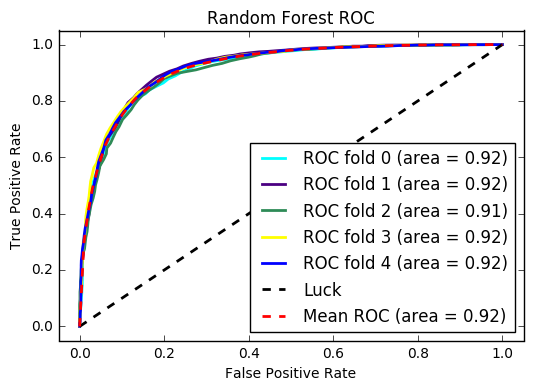
\includegraphics[width=0.9\linewidth]{rf_roc}
\caption[rf_roc]{随机森林模型交叉验证的ROC曲线}
\label{fig:rfroc}
\end{figure}

\begin{figure}[p]
\centering
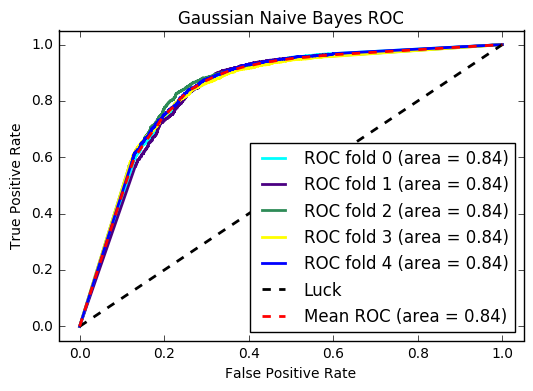
\includegraphics[width=0.9\linewidth]{gnb_roc}
\caption[gnb_roc]{高斯朴素贝叶斯模型交叉验证的ROC曲线}
\label{fig:gnbroc}
\end{figure}

\begin{figure}[p]
\centering
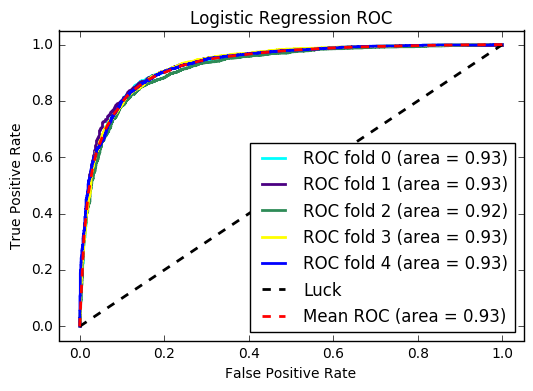
\includegraphics[width=0.9\linewidth]{lr_roc}
\caption[lr_roc]{线性回归模型交叉验证的ROC曲线}
\label{fig:lrroc}
\end{figure}

\begin{figure}[p]
\centering
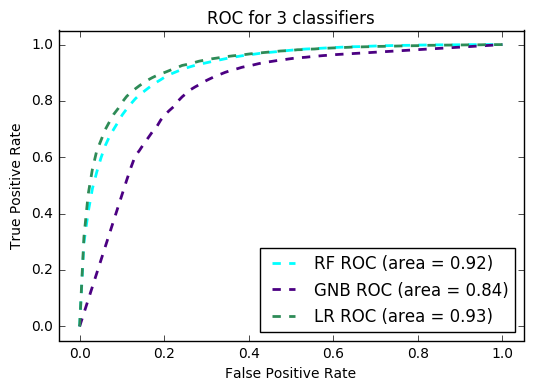
\includegraphics[width=0.9\linewidth]{3c_roc}
\caption[3c_roc]{三种模型的平均ROC曲线}
\label{fig:3croc}
\end{figure}

从三种分类器的K次交叉验证绘制出的ROC曲线来看,各个交叉验证集的ROC曲线几乎完全重合,似乎没有必要对这个数据集进行交叉验证。
另一方面,我们在实验中使用了5次交叉验证,也就是说训练时间比单个训练集测试集的方式多了4倍。
从性能和运行效率的角度考虑,我们在之后的实验中不再进行交叉验证,以节省时间。\\
在三种分类模型的横向比较中,我们发现训练过程中,随机森林的训练时间 > > 线性回归模型 > 高斯朴素贝叶斯模型。
而随机森林模型和线性回归模型的分类性能相差不大。
\paragraph{简单词包的问题}

\paragraph{简单词包的问题}
\begin{itemize}
	\item
	简单词包的方法忽略了词之间的位置关系,而只计算了词的频数。
	这样的方式缺失了上下文信息,提取的是孤立的特征。
	\item
	简单词包的方法将词包中所有的词一视同仁,没有考虑到有些词比较重要,而另一些词不是那么重要。
\end{itemize}
\paragraph{改进方式}
\begin{itemize}
	\item
	针对第一个问题,我们采用课上学到的”n-gram"的思想,将原始数据集先提取出bi-gram的特征,然后对这些特征作词包。
	\item
	针对第二个问题,我们计算文本词汇的“TF-IDF”值,作为词包集合中元素的加权值,然后将加权后的特征作为训练集测试集。
\end{itemize}

\subsubsection{基于bigram的词包}
n-gram的模型特征可以作为文本的空间信息特征。
我们仍然使用scikit-learn的CountVectorizer模块来提取词包特征,不过这时的ngram\_range参数为(2, 2),表示我们使用bigram作为词包的基本单元。\\
我们抽出前几个bigram特征:['able get',
'able make',
'able see',
'able watch',
'absolute worst',
'absolutely brilliant',
'absolutely hilarious',
'absolutely love',
'absolutely loved',
'absolutely nothing'] \\
从这几个bigram特征可以预见到提取出的特征词包中有很多像副词那样的修饰词。\\
将提取到的bigram词包特征用来训练分类器模型,得到如下图所示的ROC曲线。
\begin{figure}[h]
\centering
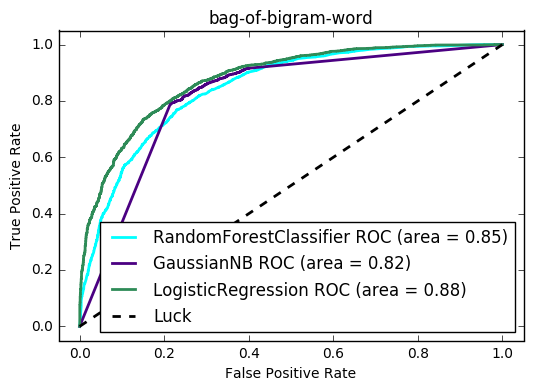
\includegraphics[width=0.9\linewidth]{3c_roc_bigram}
\caption[3c\_roc\_bigram]{三种模型用bigram词包的ROC曲线}
\label{fig:3crocbigram}
\end{figure}
从大体上我们可以看到,使用了bigram特征的分类器,其整体性能都比不使用bigram特征的分类器要差。
究其原因,我认为是像'absolutely'这样的副词修饰词占用了太多特征位置,导致其他一个词的强调词(或者那类一个词就可以鲜明地表达态度的词)没有成为词包中的频繁词,从而缺失了更有意义的特征。
	
	%----------------------------------------------------------------------------------------
	%	REFERENCE LIST
	%----------------------------------------------------------------------------------------
	\renewcommand{\refname}{参考文献}
	\begin{thebibliography}{99} % Bibliography - this is intentionally simple in this template
		
		\bibitem{1}
		
		\newblock {\em} 
		\newblock 
		
\end{thebibliography}
	
	%----------------------------------------------------------------------------------------
\end{CJK}	
\end{document}
